\section{Handover reject}
\begin{figure}[htb]
	\centering
	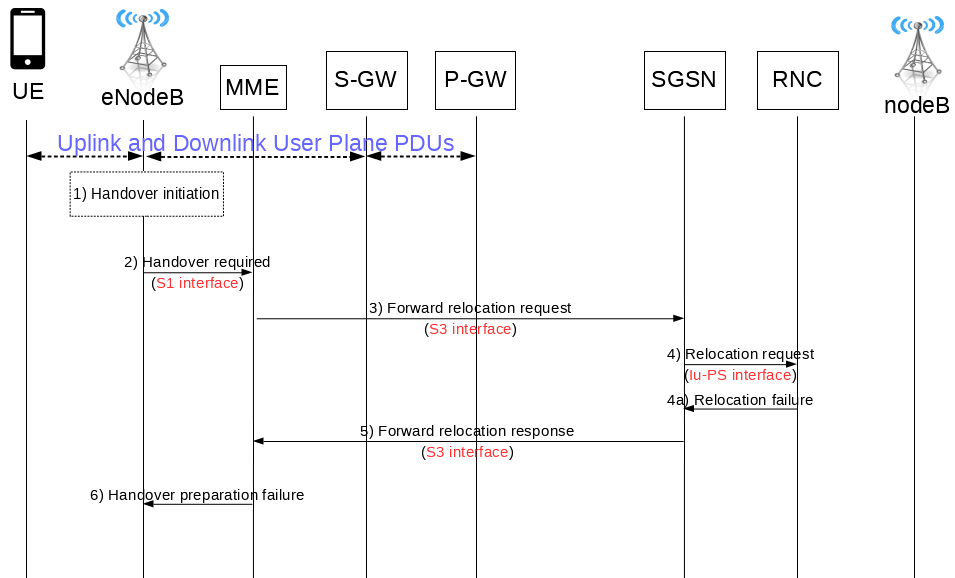
\includegraphics[width=1\linewidth]{img/handover-reject.png}
	\label{fig:preparation-phase}
\end{figure}

The Target RNC may reject the Handover if none of the RABs specified in the
Relocation Request message could be established. In this case no UE context is
established in the SGSN/RNC and no resources are allocated, the UE therefore
remains in the Source eNodeB/MME.



\subsection*{Step 1}
Step 1 to 4 are identical to the ones shown in the first chapter (Execution phase).



\subsection*{Step 4a}
The RNC fails to allocate any resources for any of the requested RABs, therefore
it sends to the SGSN a Relocation Failure message. When the SGSN receives the
Relocation Failure message it clears any reserved resources for this UE.



\subsection*{Step 5}
The SGSN sends the Forward Relocation Response message to the Source MME, specifying
the handover reject as parameter in the message (cause field).



\subsection*{Step 6}
When the MME receives the Forward Relocation Response message it sends a Handover
Preparation Failure message to the Source eNodeB.
